\begin{frame}{Modélisation}
	Deux type d'entités :
	\begin{itemize}
	\item Termes
	\item Concepts
	\end{itemize}
\end{frame}

\subsection{Une première piste}
\begin{frame}{Une première piste}{Diagramme de classes}
\begin{center}
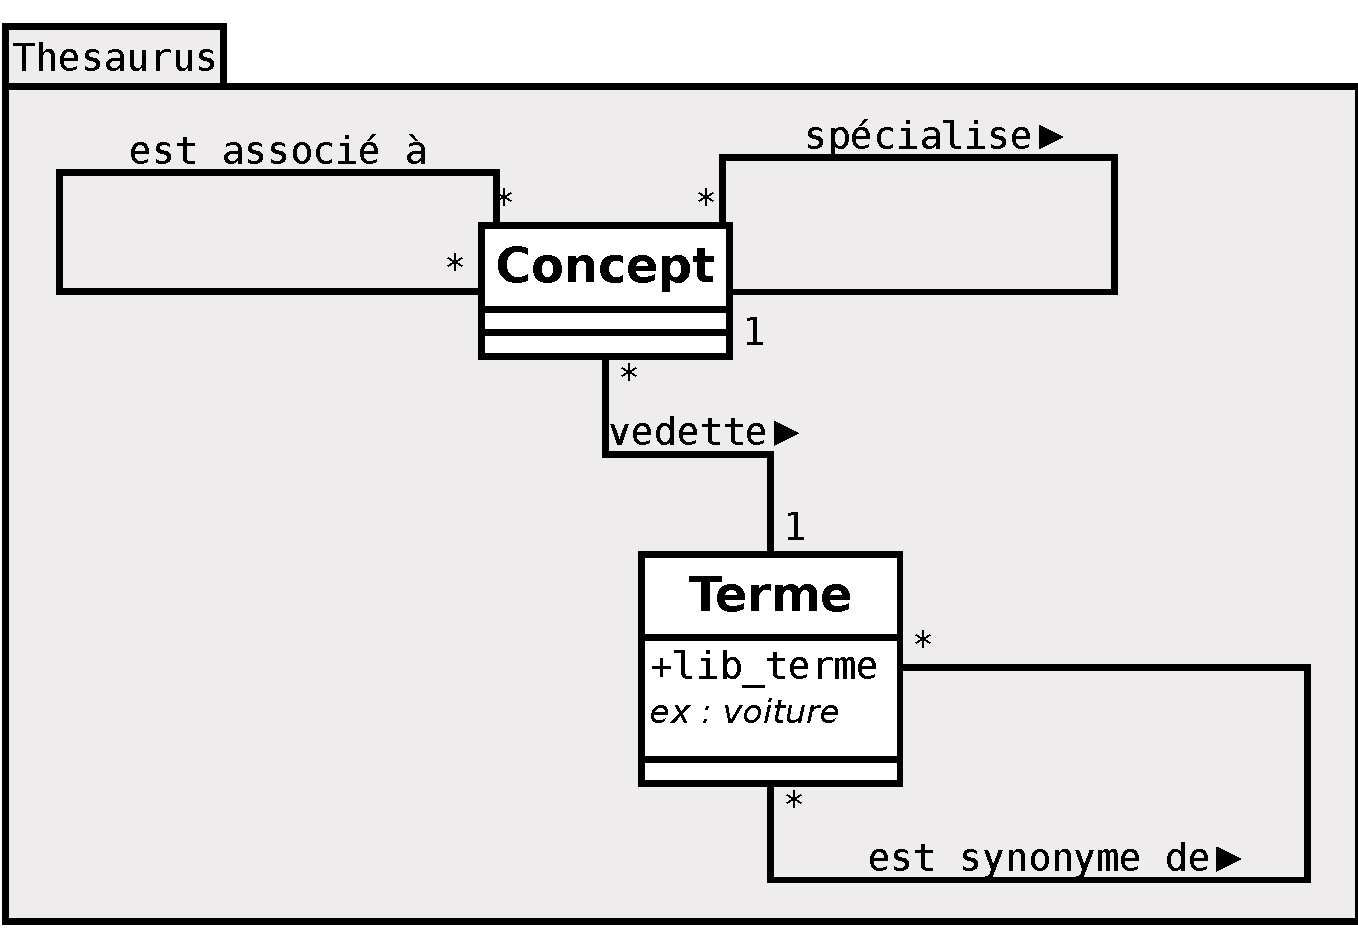
\includegraphics[width=0.5\textwidth]{files/class_v1}
\end{center}
\end{frame}

\subsection{Évolution}
\begin{frame}{Évolution}{Diagramme de classes}
\begin{center}
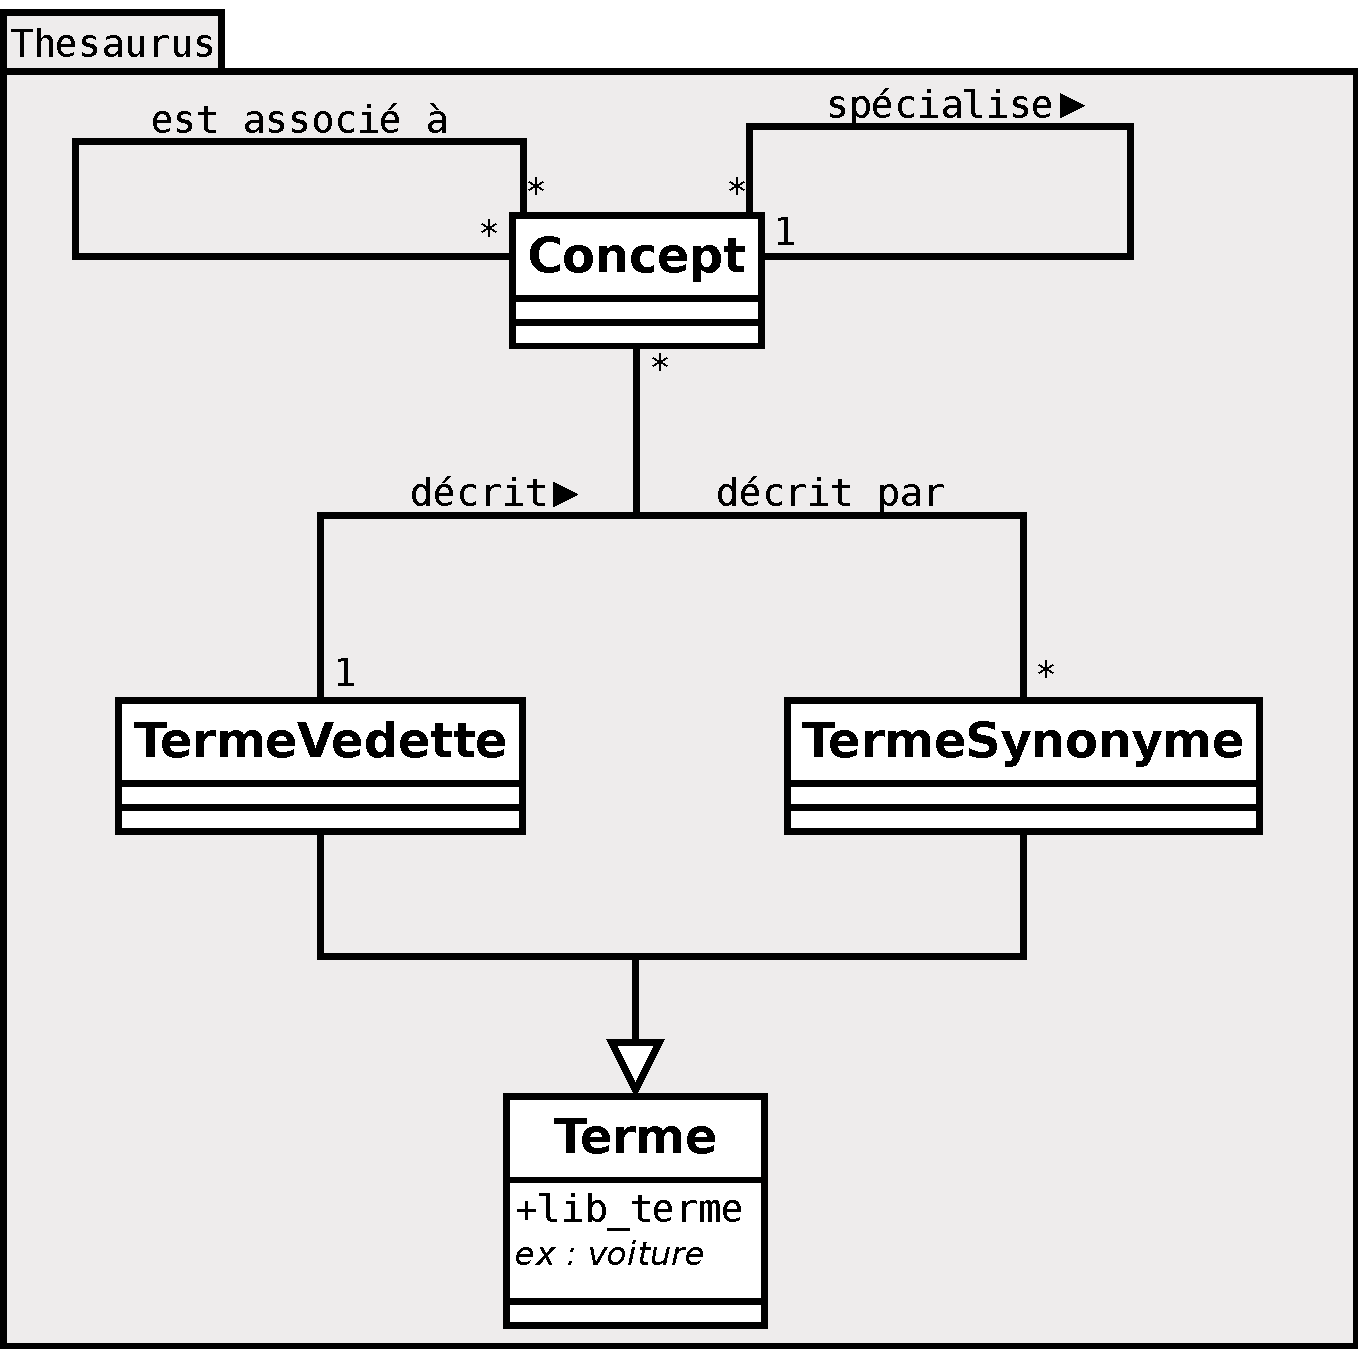
\includegraphics[width=0.5\textwidth]{files/class_v2}
\end{center}
\end{frame}

\subsection{Décision finale}
\begin{frame}{Décision finale}{Diagramme de classes}
\begin{center}
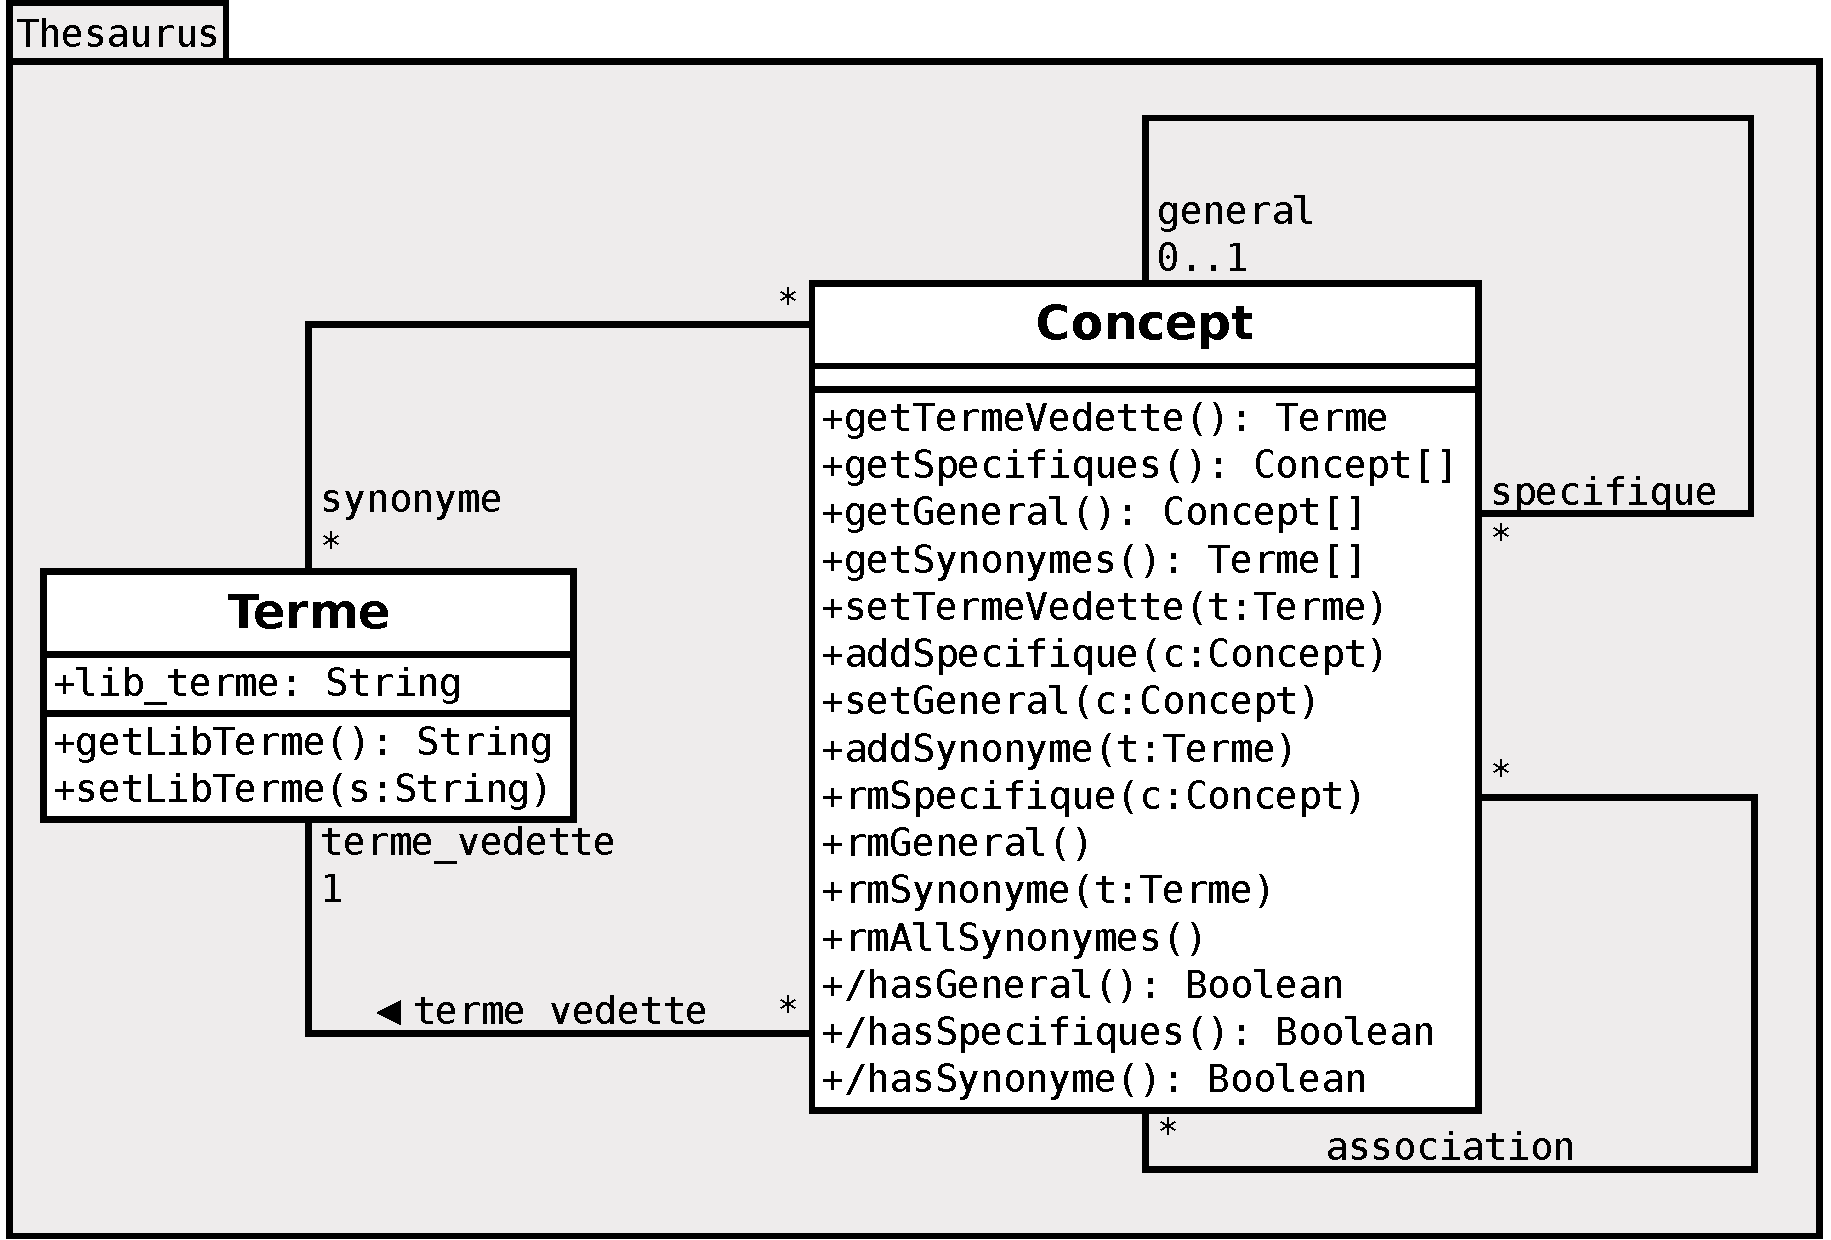
\includegraphics[width=0.6\textwidth]{files/class_v3}
\end{center}
\end{frame}
